% Latex template: mahmoud.s.fahmy@students.kasralainy.edu.eg
% For more details: https://www.sharelatex.com/learn/Beamer
\documentclass[aspectratio=169]{beamer}					% Document class

\usepackage[english]{babel}				% Set language
\usepackage[utf8]{inputenc}
\usepackage{soul}
\usepackage{bm}
\usepackage{caption}
\usetheme{Rochester}
\setbeamertemplate{navigation symbols}{}

%\usepackage[inline]{enumitem}
\usepackage{graphicx}					% For including figures
\usepackage{booktabs}					% For table rules
\usepackage{hyperref}					% For cross-referencing
\usepackage{biblatex}
\usepackage{arydshln}

\usepackage{csquotes}
\addbibresource{basu_causal.bib}
\newtheorem{assumption}{Assumption}
% myadditions
\usepackage{graphicx}
%\usepackage{enumitem}
\usepackage{bm}
\usepackage{amsfonts}
\usepackage{mathtools}
\usepackage{blindtext}
\usepackage[capitalise]{cleveref}
\usepackage{geometry}
\usepackage{graphicx,psfrag,epsf}
%\usepackage{enumerate}
%\usepackage{enumitem}
\usepackage{amssymb}
\usepackage{amsmath}
\usepackage{longtable}
\usepackage{bigints}
%\usepackage{siunitx}
\usepackage{soul}
\usepackage{tikz}
\usetikzlibrary{positioning}
\usepackage{color}

\usepackage{mathtools}
\usepackage{cleveref}
\usepackage{ragged2e}
\usepackage{etoolbox}

\apptocmd{\frame}{}{\justifying}{} % Allow optional arguments after frame.

\newcommand{\bbeta}{\bm{\beta}}
\newcommand{\hb}{\hat{\bbeta}}
\newcommand{\OLS}{\text{OLS}}
\newcommand{\sign}{\text{sign}}
\newcommand{\reals}{\mathbb{R}}
\newcommand{\naturals}{\mathbb{N}}
\newcommand{\integers}{\mathbb{Z}}
\newcommand{\Var}{\text{Var}}
\newcommand{\cdf}{F}
\newcommand{\cdfset}{\mathcal{F}}
\newcommand{\lcdf}{\underline{\cdf}}
\newcommand{\ucdf}{\overline{\cdf}}

\title[]{A Robust Bayesian Approach for Causal Inference Problems}% Presentation title

\author[]{\textbf{Tathagata Basu}, Matthias Troffaes, Jochen Einbeck}								% Presentation author			% Author affiliation
\date{ECSQARU, 2023\\

\vspace{2em}

\includegraphics[width = 0.3\linewidth]{strath_engineering.jpg}}
% Today's date	

\AtBeginSection[]
{
    \begin{frame}
        \frametitle{Table of Contents}
        \tableofcontents[currentsection]
    \end{frame}
}

\begin{document}

% Title page
% This page includes the information defined earlier including title, author/s, affiliation/s and the date
\begin{frame}
  \titlepage
\end{frame}

\section{Introduction}

\subsection{Causal Inference}

\begin{frame}{Causal Inference}
Let
\begin{itemize}
    \item $Y=(Y_1, \dots, Y_n)$ be $n$ outcomes
    \item $T=(T_1, \dots, T_n)$ be $n$ corresponding treatment indicators
\end{itemize}

In \alert{Causal Inference}, we are interested in the
\alert{treatment effect} given by: 
\begin{align}
	\delta = \mathbb{E}(Y\mid T =1) - \mathbb{E}(Y\mid T=0).
\end{align}
\pause

Similarly, for the $i$-th subject, \alert{individual treatment effect} is:
\begin{align}
	\delta_i \coloneqq \mathbb{E}(Y_i\mid T_i=1) - \mathbb{E}(Y_i\mid T_i=0).
\end{align}
\end{frame}
\iffalse
That is, the difference between the outcomes when $i$-th subject receives
the \alert{treatment} and when $i$-th subject remain as a \alert{control}. 
%\end{frame}

%\begin{frame}{Estimation}
In theory, both $\alert{\mathbb{E}(Y_i\mid T_i=1)}$ and 
$\alert{\mathbb{E}(Y_i\mid T_i=0)}$ exist.
However, we can not observe them simultaneously for the $i$-th individual. 

\vspace{2em}

Instead, we estimate the average causal effect of the treatment $T$ by 
\begin{align}
	\hat{\delta} \coloneqq 
	\frac{\sum_{i=1}^n Y_i\cdot\mathbb{I}(T_i=1) - 
		\sum_{i=1}^n Y_i\cdot\mathbb{I}(T_i=0)}{n}.
\end{align}
\fi


\begin{frame}{}
    
\end{frame}
\subsection{Regression Model}

\begin{frame}{Outcome Model}
Regression methods can reduce the
correlation between the treatment indicator and noise
\footfullcite{winship99}. 

\vspace{1em}

Let
\begin{itemize}
    \item $X\coloneqq$ $[X_1, \dots, X_n]^T$ be $p$ dimensional inputs (predictors)
    \item $\beta \coloneqq (\beta_1$, \dots, $\beta_p)^T$ be regression coefficients
    related to inputs
    \item $\beta_T$ be the regression coefficient related to the treatment
\end{itemize}

Let $\epsilon_i\sim \mathcal{N}(0, \sigma^2)$ then
we have the following \alert{outcome model} 
\begin{equation}
	Y_i =  T_i \beta_{T} + X_i\beta + \epsilon_i
\end{equation}

\end{frame}


\begin{frame}{Treatment Model}{Confounding}
In the presence of \alert{confounders}, we also need to consider the
\alert{association between the treatment indicators and the predictors}.

\begin{figure}[h]
	\centering
	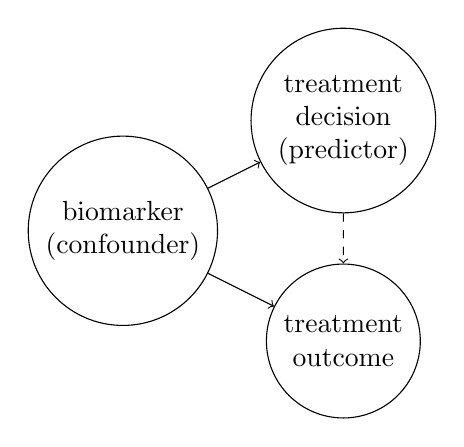
\begin{tikzpicture}[node distance=2cm, auto, scale = 0.7]
  \node (confounder) at (0,0) [circle,draw,align=center] {biomarker \\(confounder)};
  \node (predictor) at (4,2) [circle,draw,align=center] {treatment \\ decision \\ (predictor)};
  \node (outcome) at (4,-2) [circle,draw,align=center] {treatment \\ outcome};
  \draw[->] (confounder) to (predictor);
  \draw[->] (confounder) to (outcome);
  \draw[->,dashed] (predictor) to (outcome);
\end{tikzpicture}
	\caption{Confounding in causal models.}
	\label{fig:confounding}
\end{figure}

\end{frame}


\begin{frame}{Treatment Model}{Probit Link}


We can use a \alert{probit link} function to 
construct the treatment model. 

Let 
\alert{$\gamma\coloneqq(\gamma_1, \cdots, \gamma_p)$}
be a vector of regression coefficient. Then
\begin{align}
	P(T_i=1\mid X_i) = \Phi(X_i\gamma)
\end{align}
where $\Phi(\cdot)$ is the \alert{CDF}
of a standard normal distribution. 
We assume that we can model the $T_i$ through the following 
\footfullcite{albert93} latent variables:
\begin{align}
    T_i^* &= X_i\gamma +u_i; \quad u_i\sim\mathcal{N}(0,1)\\
    T_i   &= \mathbb{I}(T_i^*>0)
    =
    \begin{cases}
    1 & \text{if }T_i^*>0 \\
    0 & \text{otherwise}.
    \end{cases}
\end{align}
\end{frame}

\iffalse


\begin{frame}{Combined Model}

Let $W\coloneqq\left(\begin{smallmatrix}Y \\ \alert{T^*}\end{smallmatrix}\right)$
$X_O = [T, X]$, $X_T = X$ and 
\begin{align}
	Z &\coloneqq
	\begin{bmatrix}
		X_O & 0 \\
		0 & X_T
	\end{bmatrix}\nonumber.
\end{align}
Using Gaussianity of the measurement noise we have the \alert{joint likelihood}
\begin{align}
	W\mid Z, \alpha, \beta, \gamma, \sigma^2 \sim\mathcal{N}\left(Z\nu, \Sigma\right)\label{eq:like:group},
\end{align}
where $\nu = (\beta_T, \beta, \gamma)^T$ and
\begin{align}
	\Sigma &=
	\begin{bmatrix}
		\sigma^2{I}_n & 0 \\
		0 & {I}_n
	\end{bmatrix}\nonumber.
\end{align}

\end{frame}
\fi

\section{Bayesian Analysis}
\subsection{Spike and Slab Group LASSO}

\begin{frame}{Hierarchical Model}{Spike and 
Slab Group LASSO Prior \footfullcite{ishwaran2005}}
Let  
\begin{equation}
	\alert{\pi_j = P\left((\beta_j,\gamma_j)\not=(0,0)\right)}.
\end{equation}
So that
\begin{align}
	(\beta_j,\gamma_j)^T \mid \pi_{j}, \sigma^2 
        &\sim  \alert{\pi_{j}}
        \mathcal{N}\left( \begin{bmatrix}
		0 \\
		0
	\end{bmatrix}, 
	\tau_1^2\begin{bmatrix}
		\sigma^2 & 0 \\
		0 & 1
	\end{bmatrix}\right) 
        + \alert{(1-\pi_{j})} \mathcal{N}\left(\begin{bmatrix}
		0 \\
		0
	\end{bmatrix}, 
	\tau_0^2\begin{bmatrix}
		\sigma^2 & 0 \\
		0 & 1
	\end{bmatrix}\right)
	\\
	\beta_T\mid \sigma^2 &\sim \mathcal{N}\left(0, \sigma^2\right)\\
	%\gamma_0 &\sim \mathcal{N}(0,1)\\
	\frac{1}{\sigma^2}&\sim \text{Gamma}(a, b)\\
	\pi_{j} &\sim\text{Beta}\left(sq, s(1-q)\right).
\end{align}
\end{frame}

\iffalse
\begin{frame}{Spike and Slab Group LASSO}{Hyperparameter Specifications}

For the regression coefficients ($\beta_j,\gamma_j$)
\begin{itemize}
    \item Fix \alert{sufficiently small $\tau_0$} $(1\gg\tau_0>0)$ for 
    \alert{spike component}
    \item Fix \alert{$\tau_1$ to be large} so that $\tau_1\ge 1$ for 
    \alert{slab component}
\end{itemize}

For the \alert{precision term} ($1/\sigma^2$)
\begin{itemize}
    \item Fix \alert{$b = 1$}
    \item Elicit \alert{$a$} which represents the \alert{prior expectation} of the precision 
\end{itemize}

For the \alert{prior selection probability} ($\pi_j$)
\begin{itemize}
    \item Fix \alert{$s=1$}
    \item Elicit \alert{$q$} which represents \alert{prior expectation} of the selection probability
\end{itemize}

\end{frame}


\fi
\begin{frame}{Spike and Slab Group LASSO}{Illustration}

\begin{figure}[h]
	\begin{center}
		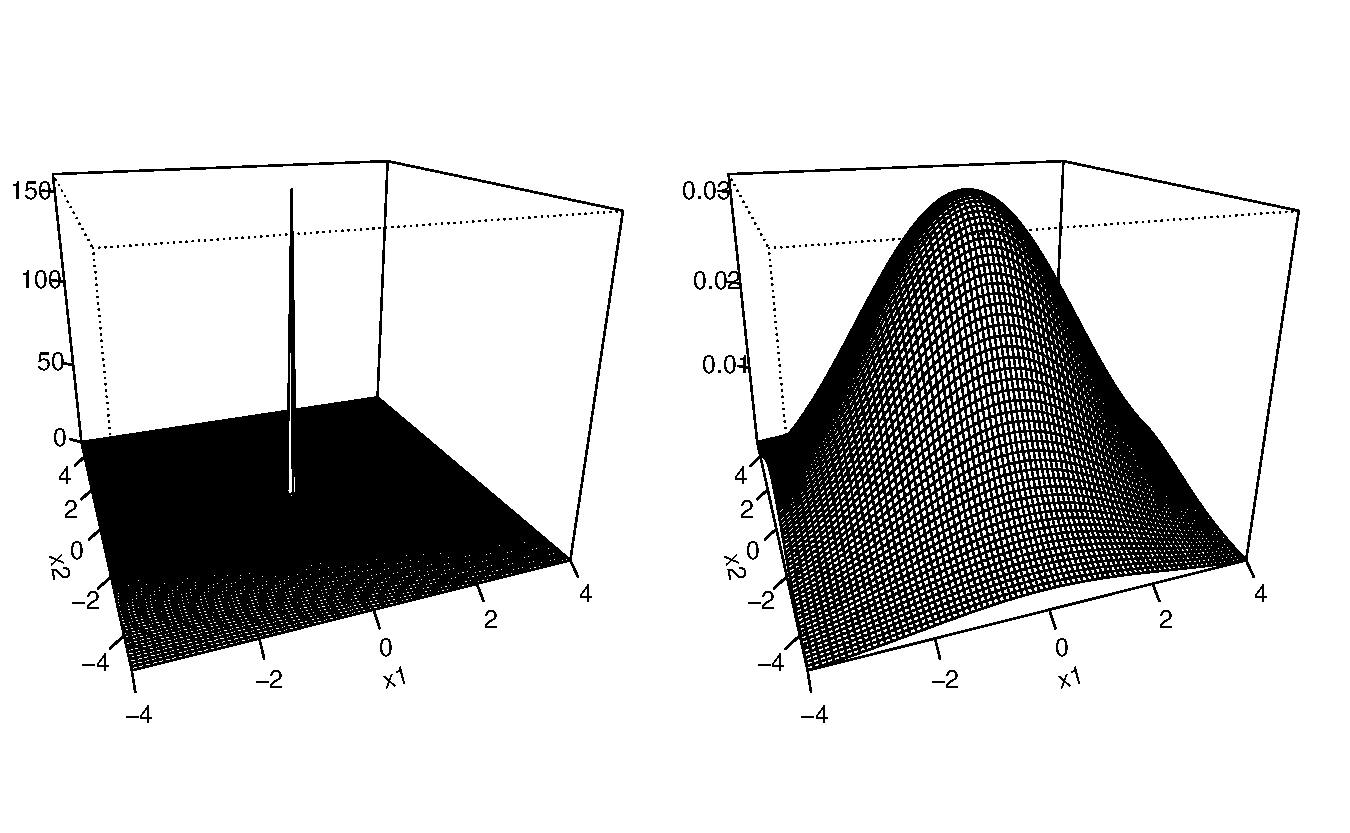
\includegraphics[width = 0.65\linewidth]{spike_slab_bi.pdf}
	\end{center}
	\caption{Spike (left) and slab (right) LASSO prior with $\tau_0 = 0.001$, $\tau_1$ = 5 and $\sigma=1$.}
	\label{fig:ssbl}
\end{figure}


\end{frame}

\subsection{Prior Sensitivity Analysis}

\begin{frame}{Elicitation}{Graphical Model}
\begin{figure}
	\centering
	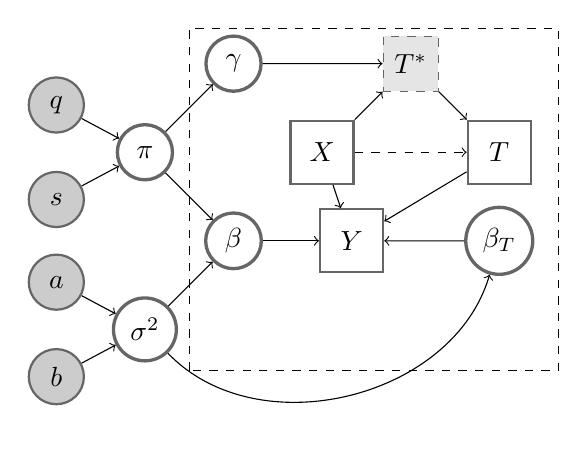
\begin{tikzpicture}[params/.style={circle, draw=black!60, very thick, minimum size=7mm},
		hyper/.style={circle, draw=black!60, fill=black!20, thick, minimum size=7mm},
		post/.style={circle, draw=black!60, fill=green!20, thick, minimum size=7mm},
		latent/.style={rectangle, draw=black!60, fill=black!10, dashed, minimum size=7mm},
		data/.style={rectangle, draw=black!60, thick, minimum size=8mm},
  scale = 0.75]
		\node[params] (1) at (0,0) {$\pi$};
		\node[data] (2) at (3,0) {$X$};
		\node[data] (3) at (6,0) {$T$};
		\node[params] (4) at (1.5,1.5) {$\gamma$};
		\node[latent] (5) at (4.5,1.5) {$T^*$};
		\node[params] (6) at (1.5,-1.5) {$\beta$};
		\node[data] (7) at (3.5,-1.5) {$Y$};
		\node[params] (8) at (0,-3) {$\sigma^2$};
		\node[params] (10) at (6,-1.5) {$\beta_T$};
		\node[hyper] (11) at (-1.5,-.8) {$s$};
		\node[hyper] (12) at (-1.5,.8) {$q$};
		\node[hyper] (13) at (-1.5,-2.2) {$a$};
		\node[hyper] (14) at (-1.5,-3.8) {$b$};
		\draw[black, dashed] (0.75,-3.7) rectangle (7,2.1);
		
		\path (1) edge[->]  (6);
		\path (1) edge[->]  (4);
		\path (8) edge[->]  (6);
		\path (6) edge[->]  (7);
		\path (2) edge[->]  (7);
		\path (2) edge[->]  (5);
		\path (5) edge[<-] (4);
		\path (5) edge[->] (3);
		\path (3) edge[->]  (7);
		\path (10) edge[->]  (7);
		\path (2) edge[dashed][->] (3);
		\path (8) edge[bend right = 60][->]  (10);
		\path (11) edge[->]  (1);
		\path (12) edge[->]  (1);
		\path (13) edge[->]  (8);
		\path (14) edge[->]  (8);
		
	\end{tikzpicture}
	\caption{Probabilistic graphical representation for causal inference.}
	\label{fig:regress}
\end{figure}

\end{frame}

\begin{frame}{Elicitation}{Possible Strategies}
Elicitation of \alert{noise}
\begin{itemize}
    \item Empirical Bayes approach and obtain an estimate for $a$
    \item Scale the dataset and fix $a=10$
\end{itemize}

Elicitation of \alert{selection probability}
\begin{itemize}
    \item Compute the marginal correlation of the inputs w.r.t. the 
    outcome %and fix the number of active variables based on a threshold. 
    \item Collect expert opinion on the relevance of the inputs.
\end{itemize}

\end{frame}

\begin{frame}{Elicitation}{Issues}
\begin{itemize}
    \item Marginal correlation may not be reliable in case of
    \alert{limited data}
    \item Causal data obtained from health sector is inherently \alert{heteroskedastic}
    \item Outcome of an unsuccessful treatment can be \alert{severe (death for instance)}.
\end{itemize}    
\end{frame}

\begin{frame}{Prior Sensitivity Analysis}
    Instead of a single value for $q$, we take a \alert{set} to
    represent \alert{bounds on the quotient of active variables} 
    \begin{equation}
        q \in \alert{\left[\underline{q}, \overline{q}\right]}\coloneqq
        \mathcal{P}\subseteq (0,1)
    \end{equation}
    So, \alert{$p\underline{q}$} and \alert{$p\overline{q}$} represents the
    lower and upper bounds of the number of active variables.

\end{frame}

\begin{frame}{Robust Decision Making}{Loss Function for Abstention}
    
We associate \alert{a loss function for abstention} (ie.~the cost of further experiments). 
\begin{table}[h]
    \caption{Losses with respect to different types of variable selection}
    \label{tab:loss:vs}
    \centering
    \begin{tabular}{l|ccc}
       &  False Positive & False Negative & Abstention \\
       \hline
       Value  &  $\ell_1$ & $\ell_2$ & $\ell_3$
    \end{tabular}
\end{table}
In most cases, $\ell_3\ll \ell_1,\ell_2$. 

\end{frame}

\iffalse
\begin{frame}{Posterior Variable Selection}{Robust Decision Rule}

The $j$-th predictor to be removed from \alert{both} the
treatment and outcome model, if
\begin{align}
	\overline{\mathbb{E}} (\pi_j\mid W)\coloneqq \sup_{q\in \mathcal{P}} \mathbb{E}(\pi_j\mid W) < 1/2.
\end{align}
Similarly, the $j$-th predictor to be present in at least one of the models, if
\begin{align}\label{eq:vs:sel}
	\underline{\mathbb{E}} (\pi_j\mid W)\coloneqq \inf_{q\in \mathcal{P}} \mathbb{E}(\pi_j\mid W) \ge 1/2.
\end{align}
Otherwise, we consider the variable to be \alert{indeterminate}

\end{frame}

\begin{frame}{Posterior Variable Selection}{Model Fitting and Prediction}

For model fitting or prediction, we evaluate point-wise. For any fixed $q$, we define
\begin{equation}
	\alert{S(q)\coloneqq
	\left\{j : E(\pi_j\mid W) \ge 1/2\right\}.}
\end{equation}
\alert{Set containing all the variables which are active in
either of the models}

Similarly, we can compute
\begin{align}
    \mathcal{S}_*\coloneqq \left\{j:\underline{\mathbb{E}} (\pi_j\mid W)\ge1/2\right\}
    &= \bigcap_{q\in \mathcal{P}}S(q)
    \\
    \mathcal{S}^*\coloneqq \left\{j:\overline{\mathbb{E}} (\pi_j\mid W)\ge1/2\right\}
    &= \bigcup_{q\in \mathcal{P}}S(q)
\end{align}
\end{frame}
\fi

\section{Illustration}
\begin{frame}{Simulation Settings 1}
For each case $X_i\sim\mathcal{N}(0, \Sigma)$
 such that $\left[\Sigma\right]_{ij} = 0.3 ^{|i-j|}$. Then
\begin{equation}
    T_i \sim \text{Bernoulli}\left(1/(1+\exp(-X_i\gamma))\right)
    \quad\text{and}\quad
    Y_i = 4T_i + X_i\beta.
\end{equation}

\begin{itemize}
    \item Case 1: $|\gamma_j|, |\beta_j|>0$ for $j\le 10$
    \item Case 2: $|\gamma_j|>0$ for $j\le 10$ and $|\beta_j|>0$ for $j\le 15$
\end{itemize}

For both the cases, we vary the numbers of observations $n$ where
$n=25 + 5k$ for $k=0,1,2,\cdots,35$ and $p = 50$.

\end{frame}

\begin{frame}{Simulation Settings 2}
For each case $X_i\sim\mathcal{N}(0, \Sigma)$
 such that $\left[\Sigma\right]_{ij} = 0.3 ^{|i-j|}$. Then
\begin{equation}
    T_i \sim \text{Bernoulli}\left(1/(1+\exp(-X_i\gamma))\right)
    \quad\text{and}\quad
    Y_i = 4T_i + X_i\beta.
\end{equation}

\begin{itemize}
    \item Case 1: $|\gamma_j|, |\beta_j|>0$ for $j\le 10$
    \item Case 2: $|\gamma_j|>0$ for $j\le 10$ and $|\beta_j|>0$ for $j\le 15$
\end{itemize}

For both the cases, we vary the numbers of predictors $p$ where
$p=25 + 5k$ for $k=1,2,\cdots,35$ and $n=100$.

\end{frame}

\begin{frame}{Results}{Other Methods}

We compare with 3 other methods

\begin{itemize}
    \item SSCE -- Spike and Slab Causal estimator
    \item BSSCE -- Bi-level Spike and Slab Causal Estimator
    \item BSSL -- Bayesian Spike and Slab LASSO
\end{itemize}

\vspace{2em}
We use RBCE to denote our method ie.~`Robust Bayesian Causal Inference'

\end{frame}

\begin{frame}{Results}{Causal Estimate (First Scenario)}
% latex table generated in R 4.3.0 by xtable 1.8-4 package
% Wed May 24 00:50:53 2023
\begin{figure}
    \centering
    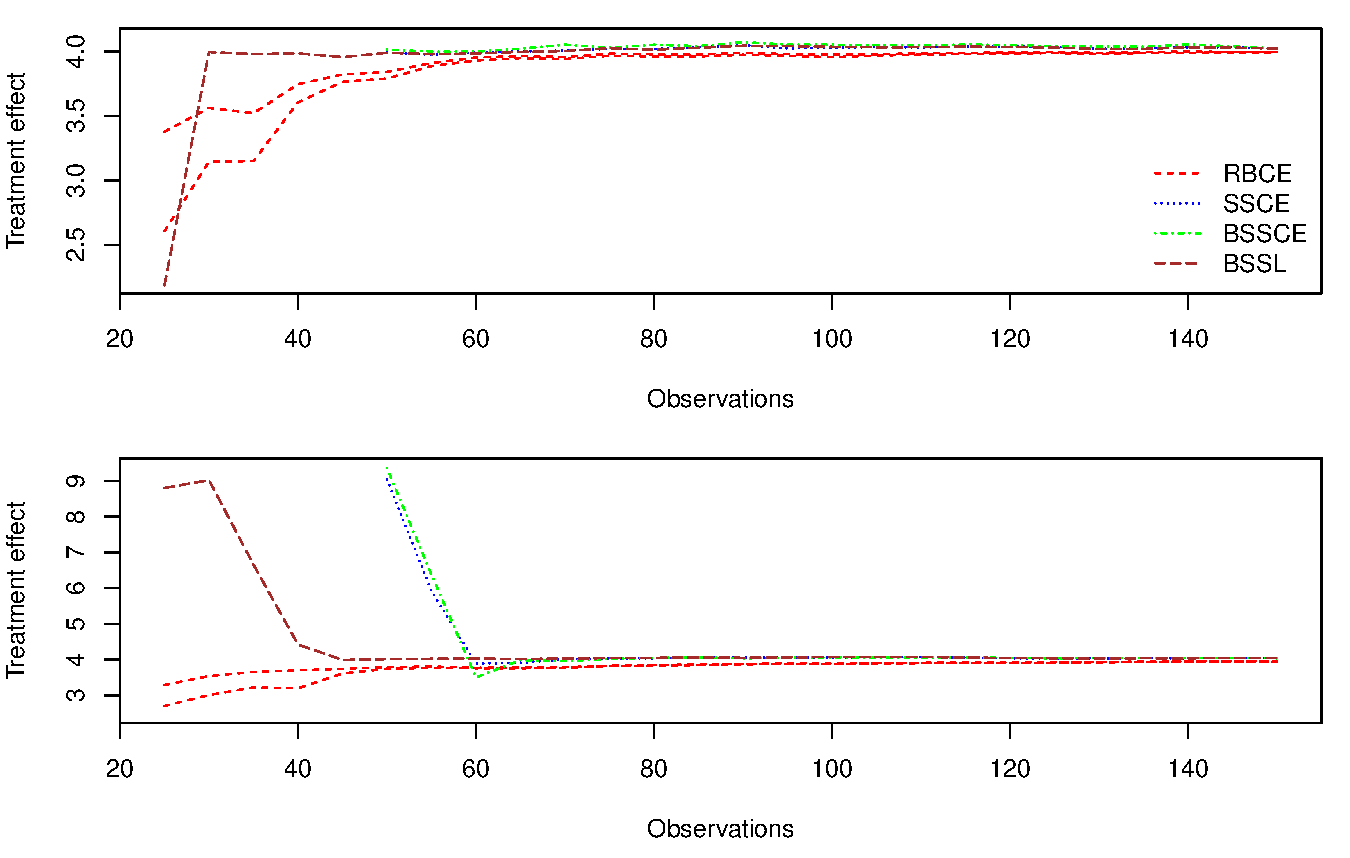
\includegraphics[width = 0.5\linewidth]{treat_obs.pdf}
    %\caption{Comparison of different methods in estimating the causal effect for varying number of observations.}
    \label{fig:comp:trt}
\end{figure}

\end{frame}

\begin{frame}{Results}{Causal Estimate (Second Scenario)}
% latex table generated in R 4.3.0 by xtable 1.8-4 package
% Tue May 23 18:29:20 2023
\begin{figure}
    \centering
    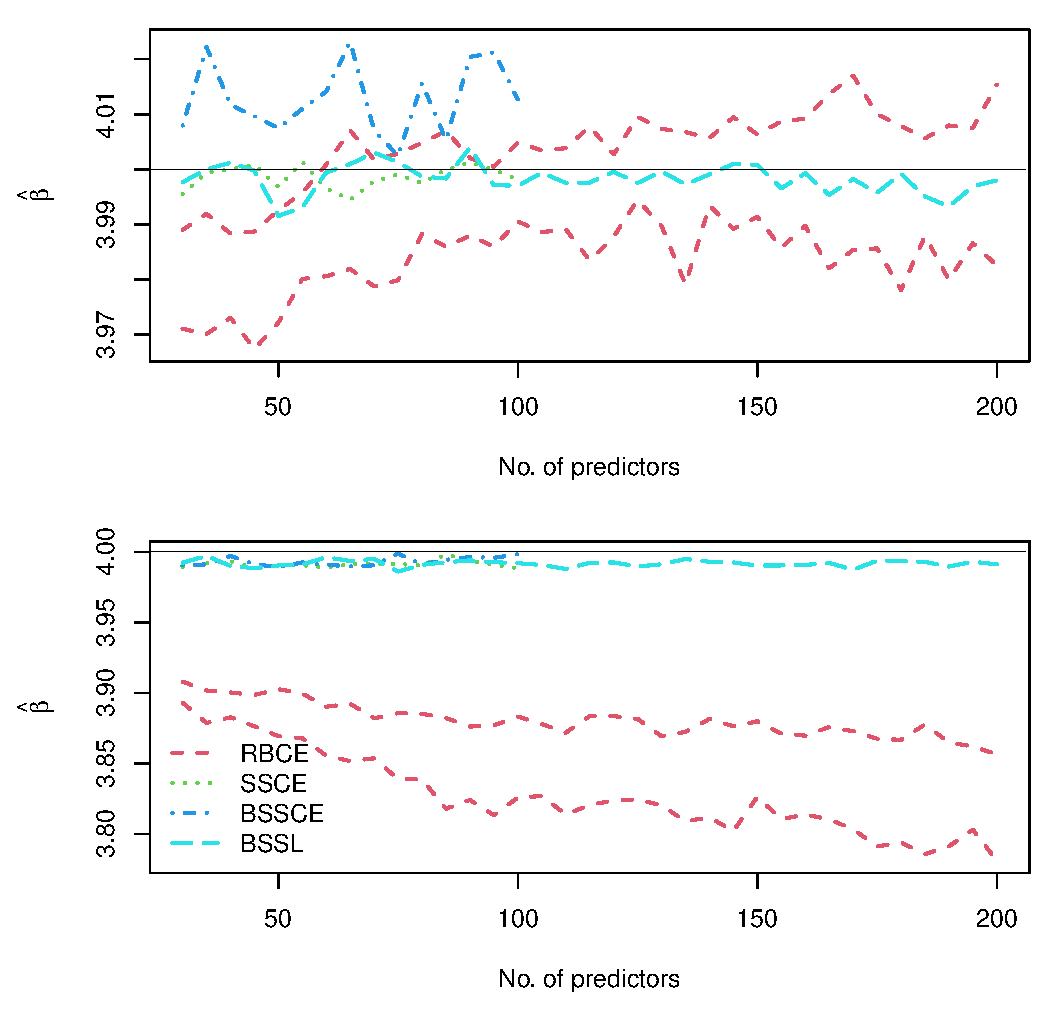
\includegraphics[width = 0.5\linewidth]{treat_pred.pdf}
    %\caption{Comparison of different methods in estimating the causal effect for varying number of predictors.}
    \label{fig:comp:trt:pred}
\end{figure}
\end{frame}

\iffalse
\begin{frame}{Results}{Causal Estimate (Graphical Comparison)}

\begin{figure}
    \centering
    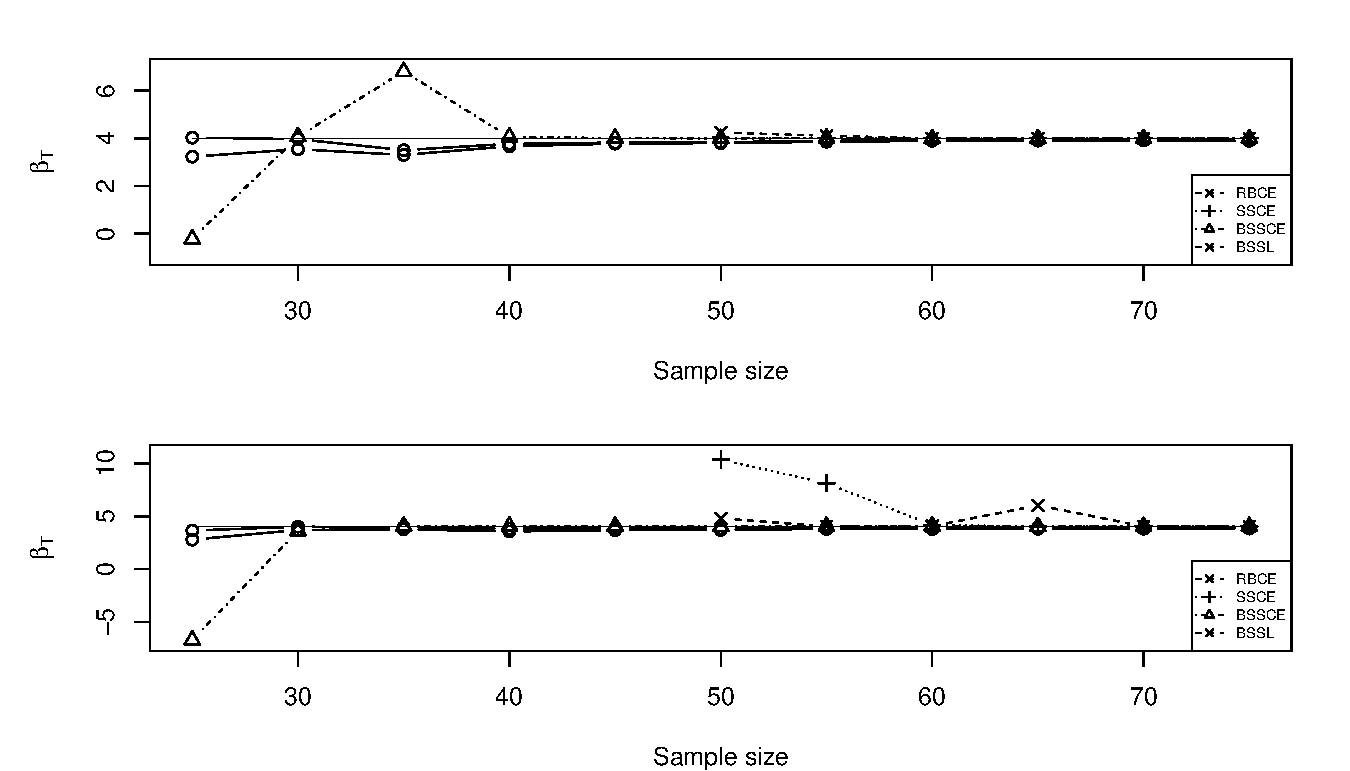
\includegraphics[width = 0.85\linewidth]{RBCE_comp.pdf}
%    \caption{Comparison of different methods in estimating the treatment effect.}
    \label{fig:comp:trt}
\end{figure}
\end{frame}

\fi
\begin{frame}{Results}{Variable Selction (First Scenario, case 1)}

Let \alert{$\ell_3 = 0.2 \ll \ell_1,\ell_2 = 1$ ($\equiv U_{80}$)}

\begin{table}[h]
    \centering
    \begin{tabular}{|c||rrr|r||rr|r||rr|r||rr|r|}
  \hline
  &\multicolumn{4}{c||}{RBCE}&\multicolumn{3}{c|}{BSSL}\\
  \cline{2-14}
 Samples & FP & FN & ID & Tot & FP & FN & Tot \\ 
  \hline
25 &   0 &   0 &  43 & 8.6 &   0 &   0&   0  \\ 
  30 &   0 &   0 &   5 & 1 &   0 &   0 &   0 \\ 
  35 &   0 &   0 &   2 & .4 &   0 &   0 &   0 \\ 
  \hline
\end{tabular}
%\caption{Covariate selection for the first three sample sizes}
\end{table}
\pause
Let \alert{$\ell_3 = 0.35, \ell_1,\ell_2 = 1$ ($\equiv U_{65}$)}

\begin{table}[h]
    \centering
    \begin{tabular}{|c||rrr|r||rr|r||rr|r||rr|r|}
  \hline
  &\multicolumn{4}{c||}{RBCE}&\multicolumn{3}{c|}{BSSL}\\
  \cline{2-14}
 Samples & FP & FN & ID & Tot & FP & FN & Tot \\ 
  \hline
25 &   0 &   0 &  43 & 15.5 &   0 &   0&   0  \\ 
  30 &   0 &   0 &   5 & 1.75 &   0 &   0 &   0 \\ 
  35 &   0 &   0 &   2 & .7 &   0 &   0 &   0 \\ 
  \hline
\end{tabular}
%\caption{Covariate selection for the first three sample sizes}
\end{table}

\end{frame}

\begin{frame}{Results}{Variable Selction (First Scenario, case 2)}

Let \alert{$\ell_3 = 0.2 \ll \ell_1,\ell_2 = 1$ ($\equiv U_{80}$)}

\begin{table}[h]
    \centering
    \begin{tabular}{|c||rrr|r||rr|r||rr|r||rr|r|}
  \hline
  &\multicolumn{4}{c||}{RBCE}&\multicolumn{3}{c|}{BSSL}\\
  \cline{2-14}
 Samples & FP & FN & ID & Tot & FP & FN & Tot \\ 
  \hline
25 &   0 &   1 &  21 & 5.2 &   0 &   0 &   0\\ 
  30 &   0 &   0 &  44 & 8.8 &  0 &  13 &   13\\ 
  35 &   0 &   0 &  11 & 2.2 &  0 &  13 &   13\\ 
  \hline
\end{tabular}
%\caption{Covariate selection for the first three sample sizes}
\end{table}
\pause
Let \alert{$\ell_3 = 0.35, \ell_1,\ell_2 = 1$ ($\equiv U_{65}$)}

\begin{table}[h]
    \centering
    \begin{tabular}{|c||rrr|r||rr|r||rr|r||rr|r|}
  \hline
  &\multicolumn{4}{c||}{RBCE}&\multicolumn{3}{c|}{BSSL}\\
  \cline{2-14}
 Samples & FP & FN & ID & Tot & FP & FN & Tot \\ 
  \hline
25 &   0 &   1 &  21 & 8.35 &   0 &   0 &   0\\ 
  30 &   0 &   0 &  44 & 15.4 &  0 &  13 &   13\\ 
  35 &   0 &   0 &  11 & 3.85 &  0 &  13 &   13\\ 
  \hline
\end{tabular}
%\caption{Covariate selection for the first three sample sizes}
\end{table}

\end{frame}

\iffalse

\begin{frame}{Results}{Variable Selction for Higher Abstention Cost (First Scenario)}

Let \alert{$\ell_3 = 0.5, \ell_1,\ell_2 = 1$}

\begin{table}[h]
    \centering
    \begin{tabular}{|c||rrr|r||rr|r||rr|r||rr|r|}
  \hline
  &\multicolumn{4}{c||}{RBCE}&\multicolumn{3}{c|}{BSSL}\\
  \cline{2-14}
 Samples & FP & FN & ID & Tot & FP & FN & Tot \\ 
  \hline
25 &   0 &   0 &  26 & 13 &  12 &   2 & 14\\ 
  30 &   0 &   1 &   1 & 1.5 &  0 &   0 & 0\\ 
  35 &   0 &   0 &   1 & 0.5 &  0 &   0 & 0\\ 
  \hline
\end{tabular}
\caption{Covariate selection for the first three sample sizes}
\end{table}


\end{frame}

\fi


\iffalse

\begin{frame}{Results}{Variable Selction (First Scenario)}

\begin{table}[h]
    \centering
    \begin{tabular}{|c||rrr|r||rr|r||rr|r||rr|r|}
  \hline
  &\multicolumn{4}{c||}{RBCE}&\multicolumn{3}{c||}{SSCE}
  &\multicolumn{3}{c||}{BSSCE}&\multicolumn{3}{c|}{BSSL}\\
  \cline{2-14}
 Samples & FP & FN & ID & Tot & FP & FN & Tot & FP & FN & Tot & FP & FN & Tot \\ 
  \hline
25 &   0 &   0 &  26 & 5.2 & -- & -- & -- & -- & -- & -- &  12 &   2 & 14\\ 
  30 &   0 &   1 &   1 & 1.2 & -- & -- & -- & -- & -- & -- &   0 &   0 & 0\\ 
  35 &   0 &   0 &   1 & 0.2 & -- & -- & -- & -- & -- & -- &   0 &   0 & 0\\ 
  40 &   0 &   1 &   0 & 1.0 &-- & -- & -- & -- & -- & -- &   0 &   0 & 0\\ 
  45 &   0 &   0 &   1 & 0.2 & -- & -- & -- & -- & -- & -- &   0 &   0 & 0\\ 
  50 &   0 &   0 &   0 & 0.0 &  0 &   0  & 0 &   0 &   0  & 0 &   0 &   0  & 0\\ 
  55 &   0 &   0 &   0 & 0.0 &   0 &   0 &   0  & 0 &   0  & 0 &   0 &   0  & 0\\ 
  60 &   0 &   0 &   0 & 0.0 &   0 &   0 &   0 &   0  & 0  & 0 &   0 &   0  & 0\\ 
  65 &   0 &   0 &   0 & 0.0 &   0 &   0 &   0 &   0 &   0  & 0  & 0 &   0  & 0\\ 
  70 &   0 &   0 &   0 & 0.0 &   0 &   0 &   0 &   0 &   0  & 0  & 0 &   0  & 0\\ 
  75 &   0 &   0 &   0 & 0.0 &   0 &   0 &   0 &   0 &   0  & 0  & 0 &   0  & 0\\ 
   \hline
\end{tabular}

\end{table}
\end{frame}

\begin{frame}{Results}{Variable Selction (Second Scenario)}

\begin{table}[h]
    \begin{tabular}{|c||rrr|r||rr|r||rr|r||rr|r|}
  \hline
  &\multicolumn{4}{c||}{RBCE}&\multicolumn{3}{c||}{SSCE}
  &\multicolumn{3}{c||}{BSSCE}&\multicolumn{3}{c|}{BSSL}\\
  \cline{2-14}
 Samples & FP & FN & ID & Tot & FP & FN & Tot & FP & FN & Tot & FP & FN & Tot \\ 
  \hline
25 &   0 &   2 &  23 & 6.6 & -- & -- & -- & -- & -- & -- &   9 &   4 & 13\\ 
  30 &   0 &   2 &   9 & 3.8 & -- & -- & -- & -- & -- & -- &   0 &   0 & 0 \\ 
  35 &   0 &   0 &  18 & 3.6 & -- & -- & -- & -- & -- & -- &   0 &   0 & 0 \\ 
  40 &   0 &   0 &   5 & 1.0 &-- & -- & -- & -- & -- & -- &   0 &   0 & 0 \\ 
  45 &   0 &   0 &   3 & 0.6 & -- & -- & -- & -- & -- & -- &   0 &   0 & 0 \\ 
  50 &   0 &   0 &   1 & 0.2 &  0 &   7 & 7 &   0 &  14 & 14 &   0 &   0 & 0 \\ 
  55 &   0 &   0 &   1 & 0.2 &  0 &   0 & 0 &  0 &  12 & 12 &  0 &   0 & 0 \\ 
  60 &   0 &   0 &   1 & 0.2 &  1 &   0 & 1 &  0 &   0 &  0 & 0 &  0 &   0 \\ 
  65 &   0 &   0 &   0 & 0.0 &  0 &  12 & 12 &  0 &   0 &  0 & 0 &  0 &   0 \\ 
  70 &   0 &   0 &   0 & 0.0 &  0 &   0 &  0 &  0 &   0 &  0 & 0 &  0 &   0 \\ 
  75 &   0 &   0 &   0 & 0.0 &  0 &   0 &  0 &  0 &   0 &  0 & 0 &  0 &   0 \\ 
   \hline
\end{tabular}
\end{table}

\end{frame}



\fi

\section{Conclusion}

\iftrue
\begin{frame}{Conclusion}
    \begin{itemize}
        \item Prior sensitivity analysis of for causal inference problem
        \item Abstention based variable selection based on generalised loss function
        \item Applicability in problems with limited information 
    \end{itemize}
\end{frame}

\fi
\begin{frame}{Future Works}
\begin{itemize}
    \iffalse
    \item Discussion of elicitation issues for causal inference models with counterfactuals
    \item Possible use of a prior sensitivity analysis for causal inference models
    \item Applicability in problems with limited information
    \pause

    \fi
    %\item \alert{Decision making with set valued estimates : Hurwicz criterion, Min-max, \dots}
    \item \alert{Inner/outer approximation strategies with MAP estimates}
    \item \alert{Monotonocity properties wrt selection probabilities \footfullcite{Basu_2022}
    for mixed models}
    \item \alert{Robust model selection with composite hypothesis testing \footfullcite{schwaferts21a}}
\end{itemize}    
\end{frame}

\begin{frame}{}
    \centering
    \huge{Thank you very much!}
\end{frame}
\begin{frame}[allowframebreaks]{References}
\printbibliography[heading=none]
\end{frame}

\end{document}
